%%%%%%%%%%%%%%%%%%%%%%%%%%%%%%%%%%%%%%%%%
% University Assignment Title Page
% LaTeX Template
% Version 1.0 (27/12/12)
%
% This template has been downloaded from:
% http://www.LaTeXTemplates.com
%
% Original author:
% WikiBooks (http://en.wikibooks.org/wiki/LaTeX/Title_Creation)
%
% License:
% CC BY-NC-SA 3.0 (http://creativecommons.org/licenses/by-nc-sa/3.0/)
%
% Instructions for using this template:
% This title page is capable of being compiled as is. This is not useful for
% including it in another document. To do this, you have two options:
%
% 1) Copy/paste everything between \begin{document} and \end{document}
% starting at \begin{titlepage} and paste this into another LaTeX file where you
% want your title page.
% OR
% 2) Remove everything outside the \begin{titlepage} and \end{titlepage} and
% move this file to the same directory as the LaTeX file you wish to add it to.
% Then add \input{./title_page_1.tex} to your LaTeX file where you want your
% title page.
%
%%%%%%%%%%%%%%%%%%%%%%%%%%%%%%%%%%%%%%%%%
%\title{Title page with logo}
%----------------------------------------------------------------------------------------
%   PACKAGES AND OTHER DOCUMENT CONFIGURATIONS
%----------------------------------------------------------------------------------------

\documentclass[12pt]{article}
\usepackage[utf8x]{inputenc}
\usepackage[T1]{fontenc}
\usepackage[francais]{babel}
\usepackage{amsmath}
\usepackage{amssymb}
\usepackage{color}
\usepackage{graphicx}
\usepackage[colorinlistoftodos]{todonotes}
\usepackage{minted}

\setlength{\parindent}{0cm} % indentation a 0 de base

\begin{document}

\begin{titlepage}

\newcommand{\HRule}{\rule{\linewidth}{0.5mm}} % Defines a new command for the horizontal lines, change thickness here

\center % Center everything on the page

%----------------------------------------------------------------------------------------
%   HEADING SECTIONS
%----------------------------------------------------------------------------------------

\textsc{\LARGE }\\[1.5cm] % Name of your university/college
\textsc{\Large Université de Nantes}\\[0.5cm] % Major heading such as course name
\textsc{\large IUT de Nantes}\\[0.5cm] % Minor heading such as course title

%----------------------------------------------------------------------------------------
%   TITLE SECTION
%----------------------------------------------------------------------------------------

\HRule \\[0.4cm]
{ \huge \bfseries Codes Correcteurs}\\[0.4cm] % Title of your document
\HRule \\[1.5cm]

%----------------------------------------------------------------------------------------
%   AUTHOR SECTION
%----------------------------------------------------------------------------------------

\begin{minipage}{0.4\textwidth}
\begin{flushleft} \large
\emph{Auteurs:}\\
Brewal \textsc{Henaff}\\
Cédric \textsc{Berland}\\
Nathan \textsc{Maraval}
\end{flushleft}
\end{minipage}
~
\begin{minipage}{0.4\textwidth}
\begin{flushright} \large
\emph{Cours:} \\
Modélisation Mathémathique % Supervisor's Name
\end{flushright}
\end{minipage}\\[3cm]


%----------------------------------------------------------------------------------------
%   DATE SECTION
%----------------------------------------------------------------------------------------

{\large \today}\\[2cm] % Date, change the \today to a set date if you want to be precise

%----------------------------------------------------------------------------------------
%   LOGO SECTION
%----------------------------------------------------------------------------------------



\includegraphics[width=4.7cm]{logo.jpg}\\%[1cm] % Include a department/university logo - this will require the graphicx package

%----------------------------------------------------------------------------------------

\newpage % Fill the rest of the page with whitespace

\end{titlepage}

%----------------------------------------------------------------------------------------
%   TABLE OF CONTENTS
%----------------------------------------------------------------------------------------
\renewcommand{\contentsname}{Sommaire}
\tableofcontents
\newpage

%----------------------------------------------------------------------------------------
%   CONFIGURATION
%----------------------------------------------------------------------------------------

\definecolor{aogreen}{rgb}{0.0, 0.5, 0.0}
\newcommand{\tab}{\hspace{1cm}}
\newcommand{\red}{\textcolor{red}}
\newcommand{\grn}{\textcolor{aogreen}}

%----------------------------------------------------------------------------------------
%   INTRODUCTION
%----------------------------------------------------------------------------------------
\section{Introduction}
\label{sec:introduction}

Ce projet à été réalisé dans le cadre de la formation en Modélisation Mathematique, en DUT Informatique à l'IUT de Nantes.

Il consiste a concevoir un programme permettant l'encodage d'un message binaire, puis par différentes methode que nous expliciterons plus tard, de le décoder et de corriger les possibles erreurs de transmission.

%----------------------------------------------------------------------------------------
%   CONTENTS
%----------------------------------------------------------------------------------------

\section{La théorie}
\label{sec:theorie}

Cette partie couvrira la théorie, les opérations effectués lors de ce projet, que ce soit lors de la transmition, ou bien de la récéption, comme du brouillage qui sera effectué pour pouvoir tester les données.

\subsection{La détection d'erreur}
\label{sub:La détection d'erreur}

Il existe plusieurs méthodes pour détecter les erreurs, par exemple associer un mot à une lettre comme utilisé dans l'armée :

\tab exemple : erreur $\rightarrow$ Echo Romeo Romeo Echo Uniforme Romeo
\\
\\ En informatique on utilise ce qu'on appel des ``bits de parité'' qui indique indique si le nombre de 1 dans l'octet est pair ou non

\tab exemple : A $\rightarrow$ 1000001 et ajoutera donc un 0 puisse que il y a deux 1 on obtiendra donc pour A le code suivant ``01000001''.
\\ Le bits de parité nous permet de savoir si lors de la transmition le message à été modifié, simplement en regardant si le bit de parité correspond toujours au reste du message (si le nombre de 1 est toujours pair).

\subsection{La correction d'erreur}
\label{sub:La correction d'erreur}

Les différents exemple ci-dessus ne permettent que de détecter les erreurs. Mais ce qui nous intéresse vraiment c'est la correction des erreurs.
\\ Il existe des moyens simple, par exemple la duplication du message :

\tab ``erreur'' $\rightarrow$ eee rrr rrr eee uuu rrr
\\ On répète chaque lettre 3 fois. Pourquoi 3 fois ? Et pas 2 ?
\\ Imaginons que l'on multiplie seulement 2 fois, on reçois le message suivant : ``ââgmee'', le message de base peut être ``âge'' mais aussi ``âme''.
\\ En revanche si l'on multiplie 3 fois on recevra donc un message tel que ``âââgmmeee'', en supposant qu'il n'y ai eu qu'une erreur, le message envoyer est donc ``âme''.

\tab Le problème de ce genre de code de correction c'est qu'ils sont très lourd, et coûteux, on transmet trois fois les données, et lorsque l'on voit le poids des données généralement transmissent (images, musiques, vidéos), on s'en rend vite compte.

\subsection{Le code de Hamming}
\label{sub:Le code de Hamming}

Depuis 1946, Richard Hamming travaille sur un système de calculateur peu fiable. En effet les données transmises sont souvent corrompus, et la machine finis invariablement par planté. C’est pour y remédier que Hamming va inventer son code correcteur.

\subsubsection{La distance de Hamming}
\label{subs:La distance de Hamming}

La distance de Hamming est une notion mathématique, évidemment défini par Hamming, qui permet de quantifier une différence entre deux séquences de symboles.
\\ Par exemple :

\tab Entre \red{0}001\red{1}1 et \red{1}001\red{0}1 on a 2 bits de différences.

\hspace{2cm} $\rightarrow$ Une distance de Hamming de 2
\\
\\ Une distance de Hamming va être applicable sur un alphabet finis, avec une même taille de bit pour tous les mots.
\\ Par exemple :

\tab 000111 et 0111 ne sont pas comparables.
\\
\\ On définit notre alphabet de taille 4, A $=$ $\{$000000; 000111; 111000; 111111$\}$
\\ La distance de Hamming fais office de code correcteur :

\tab Le mot 0000001 a une distance de 1 avec 000000, de 2 avec 000111, de 4 avec 111000, et de 5 avec 111111.
\\ Il est donc très probable que le mot reçu 000001 soit en fait le mot transmis 000000.
\\

\tab Pour utiliser la distance de Hamming, 2 notions sont importantes : la distance minimal et la capacité de correction.
\\ La distance minimal va être la distance de Hamming entre les mots de l’alphabet, et la capacité de correction va représenter le nombre de bits pouvant être détectés et corrigés.
\\

\tab Pour illustrer cela reprenons nos exemples précédents :
\\
\textbf{La duplication du message :}
\begin{enumerate}
  \item[] On reprends le cas où l’on triple chaque symbole (a $\rightarrow$ aaa)
  \item[] Notre alphabet sera A $=$ $\{$aaa; bbb; ccc; $\ldots$; ddd$\}$
  \item[] On a donc une distance minimal de 6.
  \item[] Et une capacité de correction de 1 bit : aab est corrigé en aaa.
\end{enumerate}

\linebreak
\textbf{Le bit de parité :}
\begin{enumerate}
  \item[] On a des mots de 3 bits, dont le premier est un bit de parité.
  \item[] On obtient 4 possibilités : A $=$ $\{$000; 101; 110; 011$\}$
  \item[] Cette fois la distance minimal est de 2.
  \item[] Et on a une capacité de détection de 1 bit : 001 est une erreur, cependant il est à 1 de distance entre 000 et 101, donc impossible de corriger.
\end{enumerate}

\subsubsection{Le code de Hamming}
\label{subs:Le code de Hamming}

Maintenant nous allons nous pencher sur une utilisation plus complexe et intéressante de la distance de Hamming : le code de Hamming. C’est un code correcteur actuel, dont la distance minimale est égale à trois et la capacité de correction et de 1 bit corrigé.

%%% Si possible expliqué code linéaire et code parfait %%%

\\\tab Généralement on utilise un code de Hamming C(7,4). C'est à dire que l'on envoie 7 bits et que les 4 premiers contiennent les données à transmettre. Les 3 derniers servent à la détection des erreurs.

\\\tab Il s'agit en fait d'un code correcteur parfait, c'est à dire qu'il corrige un bit avec le moins d'information possible (ici 3 bits). On peut le vérifier simplement, attention cependant on par du principe qu'il ne peut y avoir au plus qu'un bit erroné :
\begin{enumerate}
  \item[-] On a 5 états possibles : 4 états d'erreurs + 1 état sans erreur
  \item[-] On va ajouter p bits de correction, ce qui nous rajoute p états d'erreurs
  \item[-] Or p bits peuvent contenir $2^p$ informations
\end{enumerate}
\\ Ce qui nous donne l'équation à respecter :
\begin{enumerate}
  \item[$\rightarrow$] $ 5 + p = 2^p$
  \item[$\rightarrow$] Or $ 5 + 3 = 2^3$
\end{enumerate}
Ainsi C(7,4) utilise le nombre minimal de bits pour transmettre l'information tout en corrigeant une erreur.
\\
\\ Maintenant voyons comment contenir la correction dans 3 bits !
\\ Ces 3 derniers bits sont en fait l'addition, bit à bit, des 4 autres. En pratique cela donne ça :
\\ Soit $v_1, v_2, \ldots, v_7$ les bits transmit et $u_1, u_2, u_3$ et $u_4$ les bits contenant le message.
\begin{align*}
  v_1 &= u_1,\\
  v_2 &= u_2,\\
  v_3 &= u_3,\\
  v_4 &= u_4,\\
  v_5 &= u_1 + u_2 + u_4,\\
  v_6 &= u_1 + u_3 + u_4,\\
  v_7 &= u_2 + u_3 + u_4,
\end{align*}
\linebreak
\\
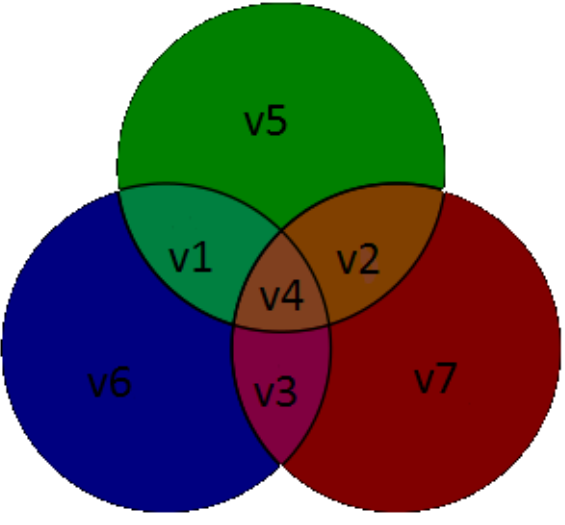
\includegraphics[width=9cm]{cercles.PNG}


Lorsque l'on reçoit le message (bits $w_1, w_2, \ldots, w_7$), on est face à 8 possibilités :

\begin{enumerate}
  \item[(0)] il n'y a pas d'erreur;
  \item[(1)] $w_1$ est erronée;
  \item[(2)] $w_2$ est erronée;
  \item[(3)] $w_3$ est erronée;
  \item[(4)] $w_4$ est erronée;
  \item[(5)] $w_5$ est erronée;
  \item[(6)] $w_6$ est erronée;
  \item[(7)] $w_7$ est erronée.
\end{enumerate}

\\ Grâce aux 3 derniers bits on peut savoir d'où provient l'erreur. Il suffit de les recalculer (bits $W_5, W_6, W_7$) et de les comparer, pour obtenir un des huit cas précédent :

\begin{enumerate}
  \item[(0)] si $w_5 = W_5$ et $w_6 = W_6$ et $w_7 = W_7$;
  \item[(1)] si $w_5 \ne W_5$ et $w_6 \ne W_6$;
  \item[(2)] si $w_5 \ne W_5$ et $w_7 \ne W_7$;
  \item[(3)] si $w_6 \ne W_6$ et $w_7 \ne W_7$;
  \item[(4)] si $w_5 \ne W_5$ et $w_6 \ne W_6$ et $w_7 \ne W_7$;
  \item[(5)] si $w_5 \ne W_5$;
  \item[(6)] si $w_6 \ne W_6$;
  \item[(7)] si $w_7 \ne W_7$.
\end{enumerate}

Cependant ce code ne permet de détecter et corriger qu'une seule erreur. Nous allons le voir au niveau des matrices :
\\
\\ \textbf{Matrice génératrice $G_h$ :}
\\
La matrice génératrice reflète ce qui est dit plus haut : en vert on a les 4 bits du message, puis les 3 bits de corrections en rouge. L'intérêt d’une telle matrice est de pouvoir être utilisé facilement par un programme, en effet une simple multiplication matricielle suffit pour encoder le message.
Ainsi pour coder mon message M $=$ $\{1011\}$, je fais M.Gh $=$ $\{1011010\}$ $=$ C
\\ \\

\begin{align*}
  M =
  \left(
    \begin{matrix}
      1 \\
      0 \\
      1 \\
      1 \\
    \end{matrix}
  \right)
  \tab
  M.Gh =
  \left(
    \begin{matrix}
    1 & 0 & 0 & 0 \\
    0 & 1 & 0 & 0 \\
    0 & 0 & 1 & 0 \\
    0 & 0 & 0 & 1 \\
    1 & 1 & 0 & 1 \\
    1 & 0 & 1 & 1 \\
    1 & 0 & 1 & 1 \\
    0 & 1 & 1 & 1
    \end{matrix}
  \right)
  \left(
    \begin{matrix}
      1 \\
      0 \\
      1 \\
      1 \\
    \end{matrix}
  \right)
  = C =
  \left(
    \begin{matrix}
      1 \\
      0 \\
      1 \\
      1 \\
      1 \\
      0 \\
      1 \\
      0 \\
    \end{matrix}
  \right)
\end{align*}

\\
Décoder le message est très simple puisque l’on connaît les bits du message, ici les 4 premiers. C $\{1011010\}$ $\rightarrow$ M $\{1011\}$\\
\\
Il s’agit maintenant de pouvoir détecter et corriger les erreurs, pour cela on va s’aider d’une matrice de contrôle :
\\
\\ \textbf{Matrice de contrôle :}
\\
Notre matrice de contrôle doit répondre à la propriété suivante :\\
\tab M est un mot de l’alphabet si, et uniquement si H . C = 0
\\Donc on peux déjà vérifier si le message encodé est valide ou non. On va appeler \textbf{syndrome} le résultat de la multiplication matricielle entre le message reçu et la matrice de contrôle. Si le syndrome est non nul, alors on a une erreur de transmission.
\\
On appelle S le syndrome calculé avec C le message reçu :\\
\\
Si S != 0, C contient un bit erroné. \\
Le mot correct M cherché diffère de C par un mot Z tel que :\\
\tab C = M + Z\\
Il s’agit de trouver ici quel bit est représenter par chaque syndrome S, pour ensuite pour le corrigé avec le message correcteur Z.\\
Or on a :\\
\begin{enumerate}
  \item[-] M  + C = M + M +Z = Z
  \item[-] C . H = S
  \item[-] Z . H = (M + C) . H = M . H + C . H = 0 + C . H = S
\end{enumerate}
\newpage
On obtient donc le même syndrome pour le message reçu et son message correcteur, ce qui va nous permettre dans la pratique de créer un index où l’on va retenir le message correcteur associer à chaque syndrome.
Avec un Hamming (7,4), on a un syndrome de 3 bits, donc un index de taille 8. Sachant que le syndrome 0 sera toujours associer à un message correct, donc un message correcteur    Z $=$ $\{0,0,0,0,0,0,0\}$. \\
\\
Pour résumer
\begin{enumerate}
  \item[-] si le syndrome est nul, le message est bon.
  \item[-] si le syndrome est non nul, alors on regarde dans l’index le bit associé à ce syndrome et on le corrige.
\end{enumerate}
\\
\\ \textbf{bit de parité :}
\\
Comme vu précédemment on peux ajouter un bit de parité à un correcteur pour détecter des erreurs plus d’erreurs.\\
Dans notre cas présent on va passer du code de Hamming(7, 4) au code de Hamming (8,4). La distance de Hamming minimal va passer de 3 à 4, et on va pouvoir détecter 2 bits d’erreurs. \\
En effet dans le cas ou 2 bits sont modifié, on va obtenir un syndrome non nul car le message est erroné, et pourtant le bit de parité sera exact, car c’est un nombre pair d’erreur. Dans ce cas le message devra être renvoyé.\\
Cependant l’erreur est indétectable avec 3 bits erronés.\\
\\
Pour résumer
\begin{enumerate}
  \item[-] syndrome nul et bit de parité bon $\rightarrow$ pas d’erreur
  \item[-] syndrome non nul et bit de parité faux $\rightarrow$  1 erreur corrigeable par le syndrome
  \item[-] syndrome non nul et bit de parité bon $\rightarrow$ 2 erreurs, retransmission nécessaire
  \item[-] syndrome nul et bit de parité faux $\rightarrow$ 1 erreur corrigeable par le syndrome
\end{enumerate}
\newpage

\section{Notre code}
\label{sec:Notre code}

\subsection{L'envoi du message}
\label{sub:L'envoi du message}

Test de code :

\begin{minted}[linenos, frame=single]{c}
int GMatrix[4][8] = {{1,1,0,1,1,0,0,0},
                     {0,1,1,1,0,1,0,0},
                     {1,0,1,1,0,0,1,0},
                     {1,1,1,0,0,0,0,1}} ;
char G[4] ;
void init_generators() {
 for (int i=0; i < 4; ++i) {
   G[i] = 0 ;
   for (int j=0; j < 8; ++j)
     if (GMatrix[i][j]) G[i] |= (1 << (7-j)) ;
 }
}

 void hamming(char c, char out[2]) {
   out[0] = out[1] = 0;
   for (int i=0; i < 4; ++i) {
     if (c & (1 << i))
       out[1] ^= G[i] ;
     if (c & (1 << (i+4)))
       out[0] ^= G[i] ;
   }
 }


\end{minted}


\mint{c}{printf("Sur une ligne")}

\subsection{Le brouillage}
\label{sub:brouillage}

Afin de pouvoir tester notre code dans des conditions d'erreurs réelles, nous utilisons un programme permettant de brouiller certains bits, aléatoirements. Ce brouillage nous permet de tester notre code décodeur, étant donné que la probabilité d'un brouillage dû au code d'encodage est extremement faible.

Pour se faire, nous utilisons le code transmit.c, qui simule une transmition de message (comme par example l'envois d'un message à un satelite en orbite, ce qui peut engendrer de nombreuses erreurs).



\subsection{La réception et le décodage du message}
\label{sub:La réception et le décodage du message}



\section{d'assault}
\label{sec:assault}


Comments can be added to the margins of the document using the \todo{Here's a comment in the margin!} todo command, as shown in the example on the right. You can also add inline comments too:

\todo[inline, color=green!40]{This is an inline comment.}

\subsection{Tables and Figures}

Use the table and tabular commands for basic tables --- see Table~\ref{tab:widgets}, for example. You can upload a figure (JPEG, PNG or PDF) using the files menu. To include it in your document, use the includegraphics command as in the code for Figure~\ref{fig:frog} below.

% Commands to include a figure:
%\begin{figure}
%\centering
%\includegraphics[width=0.5\textwidth]{frog.jpg}
%\caption{\label{fig:frog}This is a figure caption.}
%\end{figure}

%\begin{table}
%\centering
%\begin{tabular}{l|r}
%Item & Quantity \\\hline
%Widgets & 42 \\
%Gadgets & 13
%\end{tabular}
%\caption{\label{tab:widgets}An example table.}
%\end{table}

\subsection{Mathematics}

\LaTeX{} is great at typesetting mathematics. Let $X_1, X_2, \ldots, X_n$ be a sequence of independent and identically distributed random variables with $\text{E}[X_i] = \mu$ and $\text{Var}[X_i] = \sigma^2 < \infty$, and let
$$S_n = \frac{X_1 + X_2 + \cdots + X_n}{n}
      = \frac{1}{n}\sum_{i}^{n} X_i$$
denote their mean. Then as $n$ approaches infinity, the random variables $\sqrt{n}(S_n - \mu)$ converge in distribution to a normal $\mathcal{N}(0, \sigma^2)$.

\subsection{Lists}

You can make lists with automatic numbering \dots

\begin{enumerate}
\item Like this,
\item and like this.
\end{enumerate}
\dots or bullet points \dots
\begin{itemize}
\item Like this,
\item and like this.
\end{itemize}

We hope you find write\LaTeX\ useful, and please let us know if you have any feedback using the help menu above.

%----------------------------------------------------------------------------------------
%   ANNEXES SECTIONS
%----------------------------------------------------------------------------------------
\appendix
\section{Annexe 1}
\label{sec:Annexe 1}


\end{document}
